\documentclass[a4paper,11pt]{article}

\usepackage[utf8]{inputenc}
\usepackage{mathpazo}
\usepackage{gensymb}
\usepackage{graphicx}
\usepackage{url}
\usepackage[frenchb]{babel}
\usepackage{subfig}
\usepackage[T1]{fontenc}
%% \usepackage [nottoc]{tocbibind}

\begin{document}

\title{Sorgho \& Niébé au Burkina Faso}
\author{Marilyne Aza-Gnandji}
\date{Avril 2018} 

\maketitle
\tableofcontents

\section{Situation actuelle de la production agricole au Burkina Faso}

Le Burkina Faso est un pays à économie agraire avec une population de
19\,632\,147 habitants pour une superficie de 270 764
km\textsuperscript{2} (FAO, 2017). Le secteur agricole constitue une
composante essentielle de son économie. Il contribue pour 35\% au
Produit Intérieur Brut (PIB) du pays et emploie 82\% de la population
active. L’arboriculture et le maraîchage occupent également une place
non négligeable\footnote{\url{http://agriculture.gouv.fr/burkina-faso}}
avec environ 600\,000 petites exploitations agricoles qui sont par
définition dans le recensement agricole, de petites unités de
production remplissant les trois critères suivants: produire des
produits agricoles; avoir une gestion courante indépendante; atteindre
un certain seuil en superficie (inférieur ou au moins égal à un
hectare), en production ou en nombre
d’animaux\footnote{https://www.insee.fr/fr/metadonnees/definition/c1186}.
L’agriculture burkinabé est essentiellement de subsistance et, est
basée sur les cultures vivrières (sorgho, mil, maïs, riz et fonio)
dont les rendements moyens étaient entre 2012 et 2013 d’environ 869
806 tonnes. En effet, pour la période de consommation du 1er novembre
2012 au 31 Octobre 2013, le bilan céréalier définitif fait ressortir
un excédent brut de 665 814 tonnes, résultant d’un excédent brut des
céréales traditionnelles (mil, sorgho, maïs, fonio) de 1 038 338
tonnes et des déficits bruts respectifs de 353 122 tonnes et 19 401
tonnes pour le riz et le blé (DPSAA, 2013). L’activité agricole au
Burkina Faso est menée dans des conditions parfois défavorables
(mauvaise pluviométrie, pauvreté des sols…). Ce faisant, la production
agricole est faible et ne parvient pas à couvrir les besoins
alimentaires des populations. Le Burkina Faso possède un climat
tropical de type soudano-sahélien (caractérisé par des variations
pluviométriques considérables allant d’une moyenne de 350 mm au Nord à
plus de 1\,000 mm au Sud-Ouest) avec deux saisons très contrastées :
la saison des pluies avec des précipitations comprises entre 300 mm et
1200 mm et la saison sèche durant laquelle souffle l’harmattan, un
vent chaud, sec et chargé de poussière, originaire du désert du
Sahara. La saison des pluies dure environ 4 mois, entre mai-juin et
septembre, sa durée est plus courte au nord du
pays\footnote{http://www.burkina-faso.ca/climat-du-burkina-faso/}. Le
taux de croissance de la production agricole est de l’ordre de 4,3\%
(1983 à 2007) et, selon Ngaido (2006), ce taux devrait être de 6,8\%
pour l’atteinte des Objectifs du Millénaire pour le Développement en
matière de réduction de la faim. Alors, près de 46\% de la population
totale est exposé à l’insécurité alimentaire et on estimait en 2003 le
niveau de couverture des besoins nutritionnels à 2 283 kilocalories
par personne et par jour contre les 2500 kcal requis. Parallèlement,
la pauvreté au Burkina est essentiellement rurale
(la contribution du milieu rural à la
pauvreté s’élevait à 92,2\% en 2003) et la population rurale est en
grande majorité agricole (DPSAA, 2011).  Le Burkina Faso a besoin
d’une croissance soutenue de sa production agricole non seulement pour
assurer sa sécurité alimentaire mais aussi pour lutter contre la
pauvreté et assurer son développement économique\footnote{https://www6.inra.fr/fabatropimed/FTM-Publications/FTM-Master-BTS}.
%%\cite{Mack_2007}.

\section{Productions agricoles de céréales:Le Sorgho i.e \emph{Sorghum bicolor} (L.) Moench}

%%Insérer dans un texte une référence de figure : (Fig.~\ref{images:photo_plante_sorgho})

% \begin{figure}%
  %\begin{center}
   %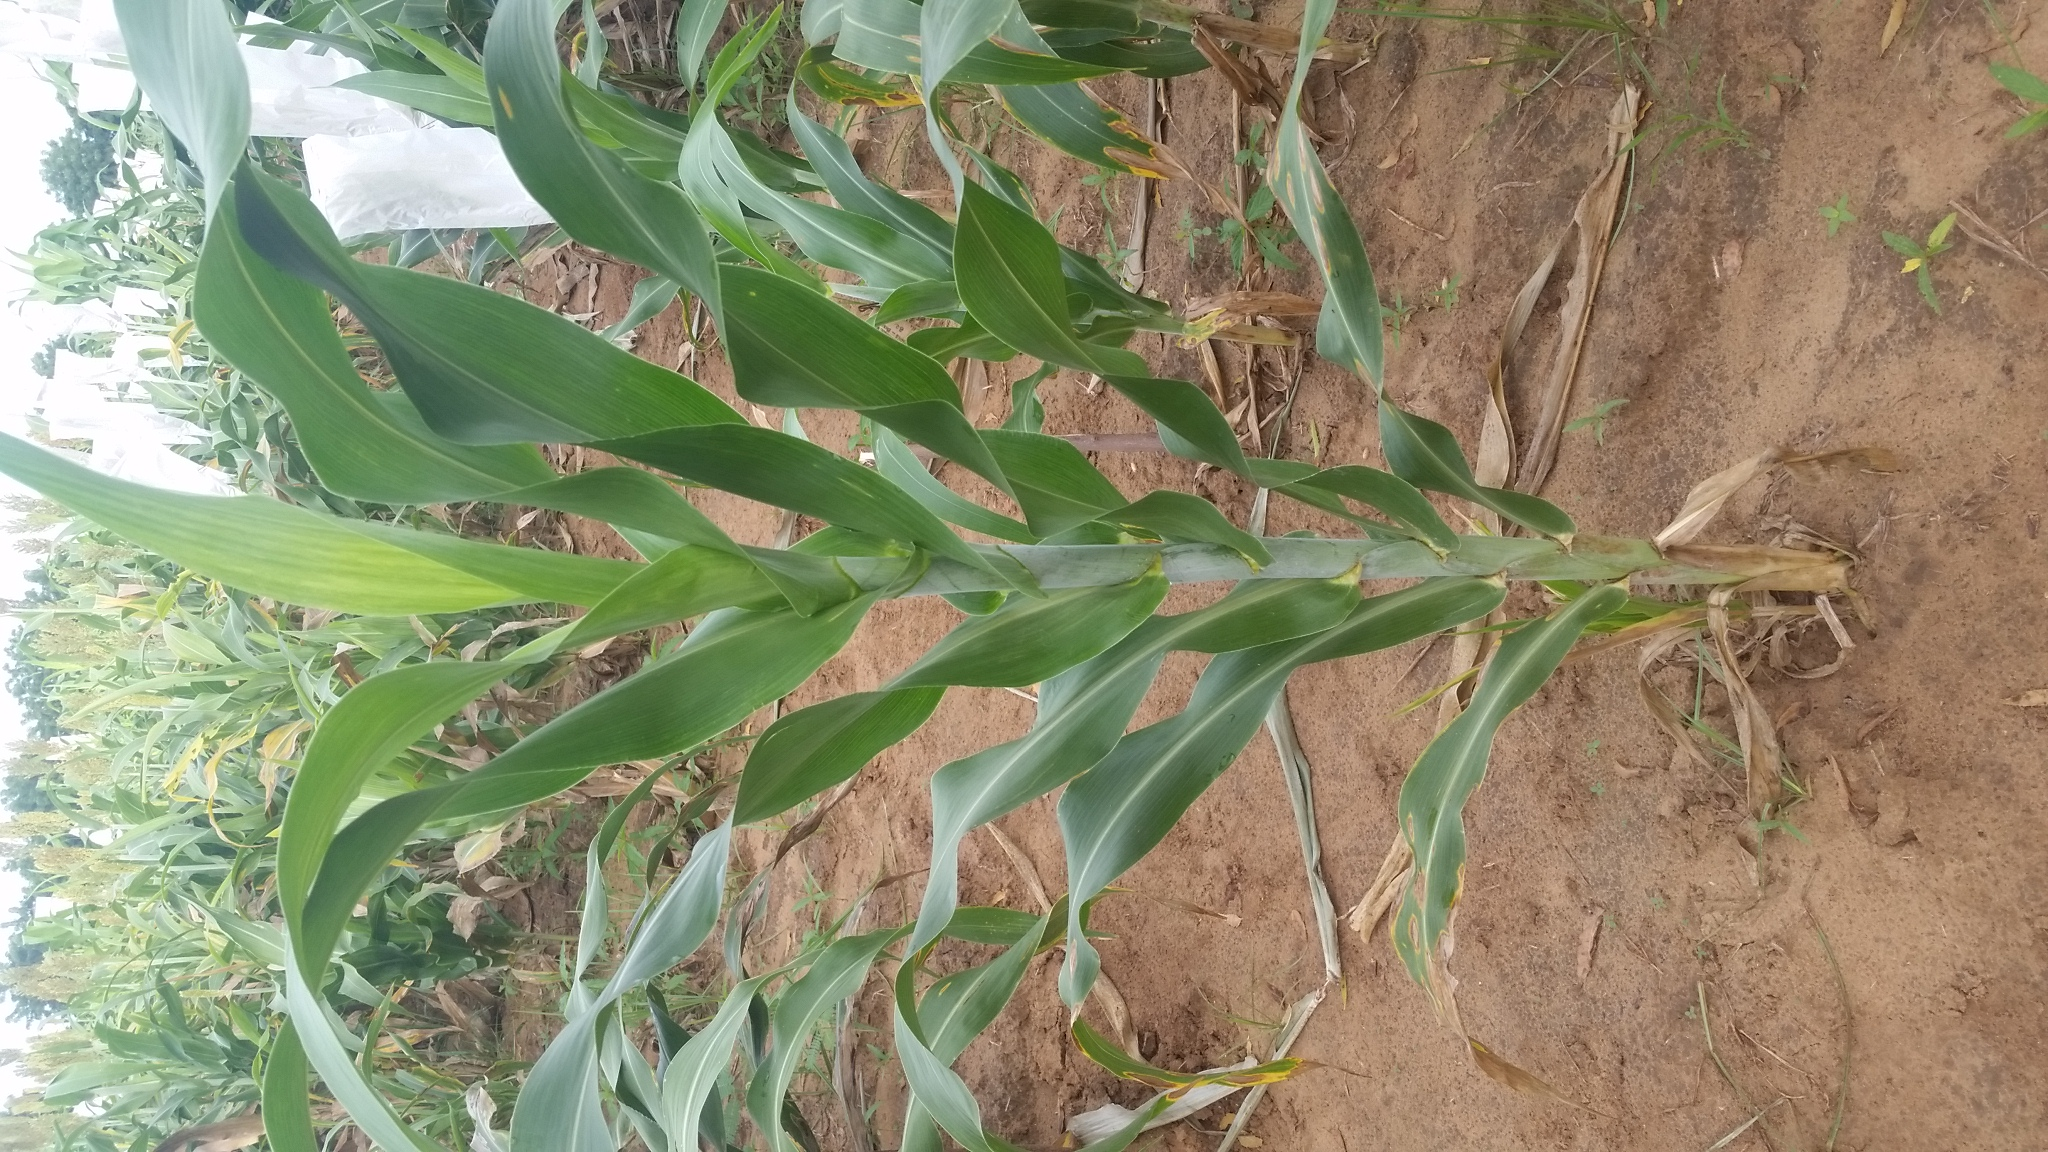
\includegraphics[width=10cm,angle=270]{images/Plante_Sorgho}
   % \end{center}
  %\caption{Plante du sorgho et quelques variétés de graine}
 % \label{images:photo_plante_sorgho}
%\end{figure}

\begin{figure}[htbp]
\begin{center}
\leavevmode
\subfloat[Plante du Sorgho]{%
\label{fig-Plante du Sorgho}
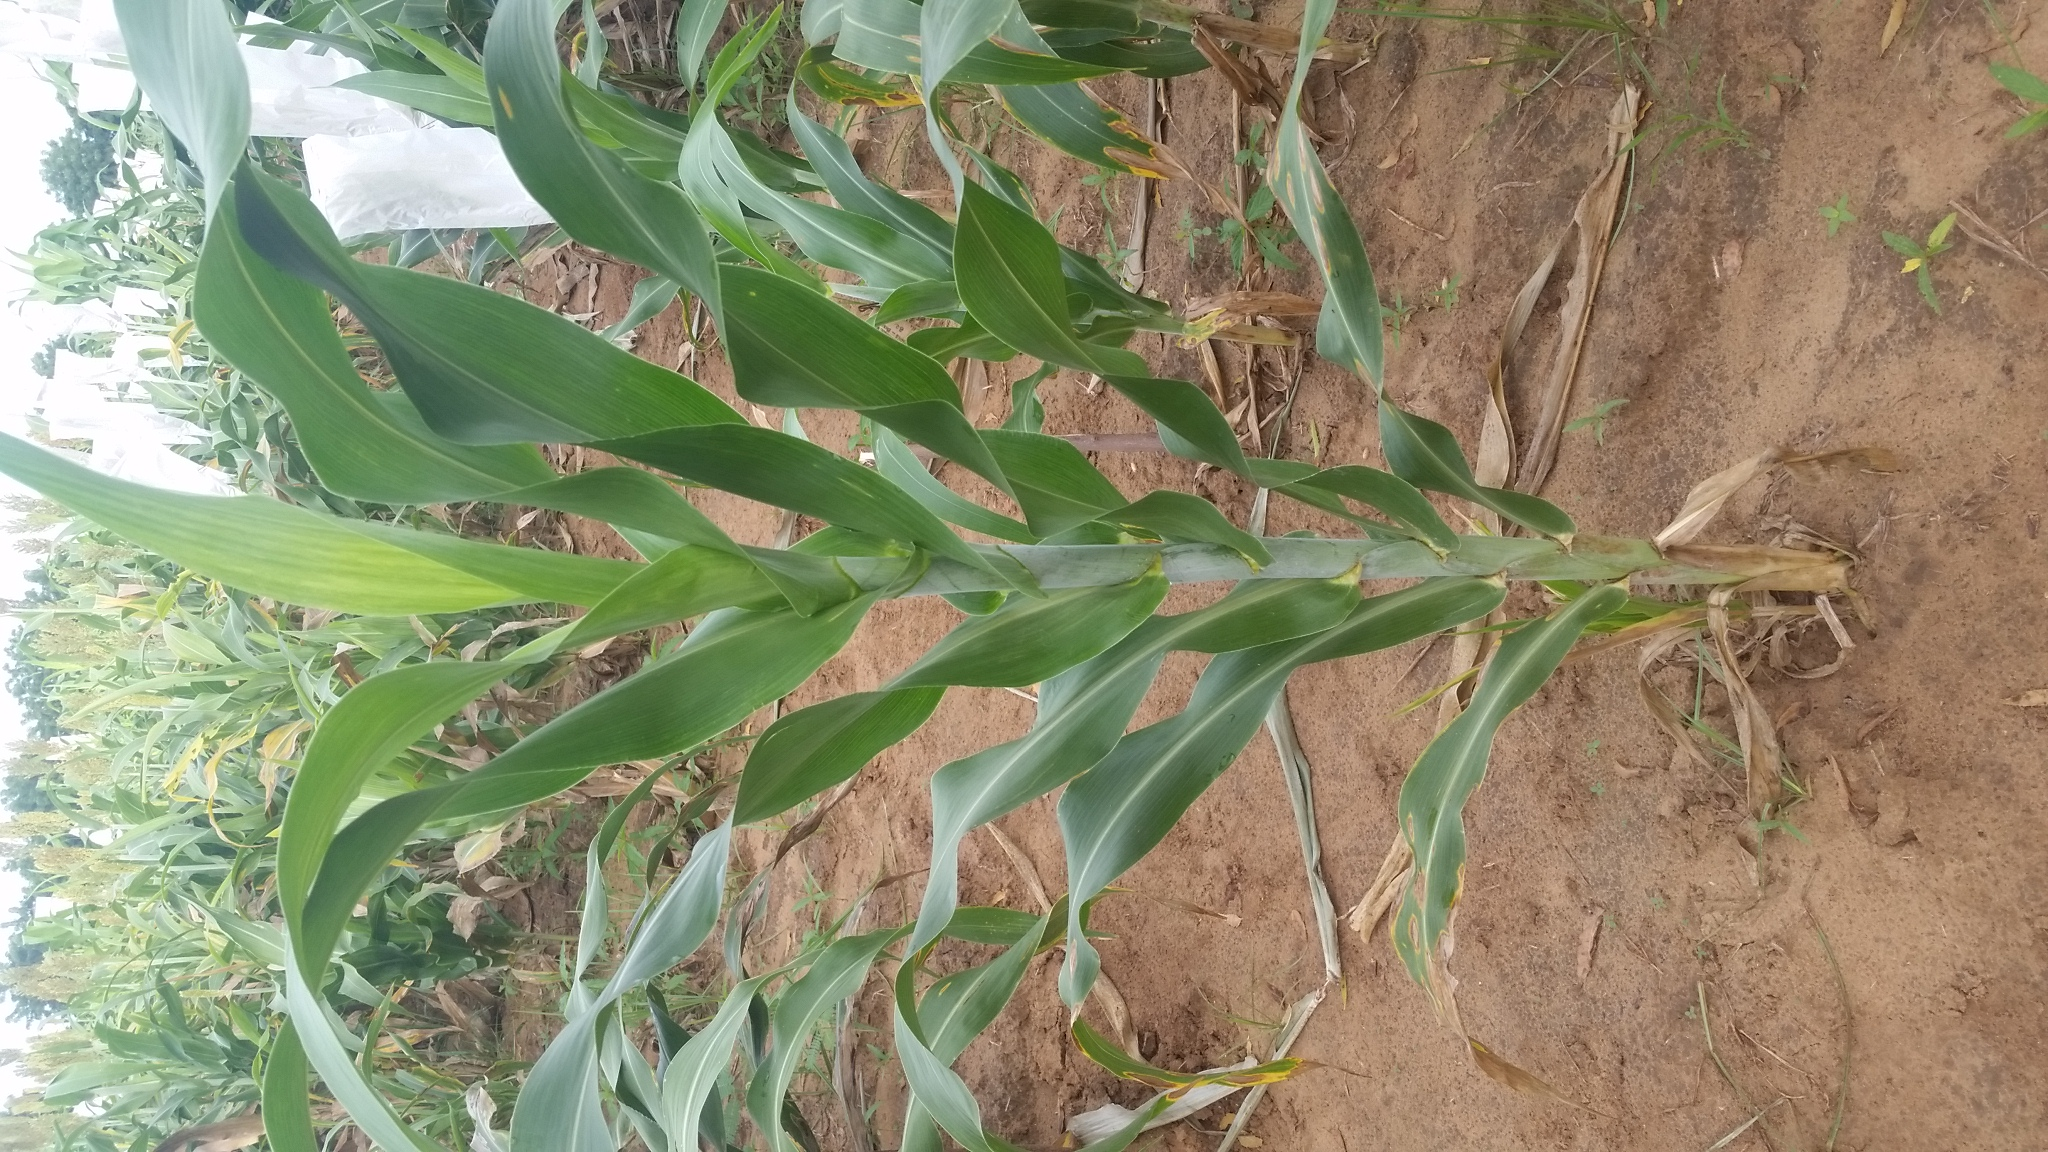
\includegraphics[width=10cm,angle=270]{images/Plante_Sorgho}}
\hspace{0.5cm}
\subfloat[Graines du Sorgho]{%
\label{fig-Graines du Sorgho}
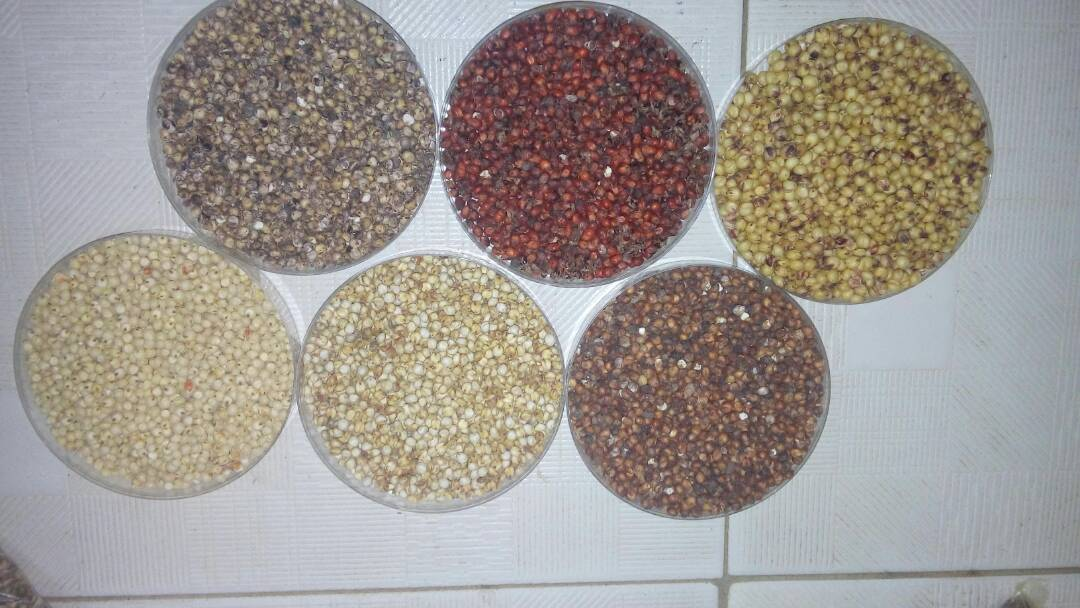
\includegraphics[width=10cm,angle=270]{images/GrainesDeSorgho}}
\caption{Plante du sorgho et quelques variétés de ses graines}
\end{center}
\end{figure}


  
\subsection{Origine \& Diffusion:}
Le sorgho est probablement originaire d’Éthiopie, d’où il s’est
répandu dans toute l’Afrique. Le sorgho commun (Sorghum bicolor) est
une graminée très répandue à l’état sauvage sous les climats tropicaux
et subtropicaux. C’est une plante de climat chaud, mais comme pour le
maïs, la sélection a permis de créer des variétés cultivables en pays
tempérés. En Europe, sa culture reste cependant cantonnée aux pays
méditerranéens (Wikipédia, 2017). Depuis des siècles, les peuples
d’Afrique et d’Asie utilisent ses graines pour leur
alimentation. Aujourd’hui, le sorgho est cultivé sur tous les
continents, sous un nom parfois différent: le gros mil en Afrique, le
millet indien en Asie ou encore le blé égyptien au Moyen-Orient. La
domestication du sorgho a vraisemblablement eu lieu il y a plusieurs
millénaires en Afrique et au Sud-est du Sahara.  On note en
Afrique\,trois centres géographiques actifs dans la diversification du
sorgho cultivé: le centre ouest-africain qui a contribué à
l’établissement des sorghos de race guinea; le centre est-africain
riche en sorgho des races caudatum et durra; le centre sud-africain à
l’origine des sorghos de race kafir. Dès le troisième millénaire
avant J.-C., ces sorghos auraient gagné l’Asie: l’Inde et le Pakistan,
3000 ans avant J.-C., puis la Chine, un millénaire plus
tard. L’arrivée du sorgho en Europe se situerait vers 2000 ans avant
J.-C. Transporté en Amérique à l’époque des grandes découvertes au
XVIe siècle, le sorgho est véritablement diffusé qu’à partir du XIXe
siècle, notamment aux
États-Unis\footnote{http://www.gnis-pedagogie.org/sorgho-intro-caracteristiques-plante.html}.

\subsection{Taxonomie:}
Le sorgho, Sorghum bicolor (L.) Moench, est une herbacée annuelle de
la famille des Poaceae (ex-Graminées), sous famille des Panicoïdeae,
tribu des Andropogoneae et du genre \emph{Sorghum}\cite{Doggett_1988}.
C’est une espèce monoïque préférentiellement
autogame. Le taux d’allogamie varie selon la race considérée: très
faible pour les variétés cléistogames qui subissent une
autopollinisation automatique ce qui traduit la caractéristique de ces
variétés de sorgho à se reproduire par autopollinisation et ainsi
leurs fleurs ne s’ouvrent qu’après l’anthèse (période terminale\,du
développement de la fleur depuis son épanouissement jusqu’au
flétrissement). Ce taux est de l’ordre de 5 à 7\% pour les variétés à
panicules compactes (Doggett, 1988), et varie largement (20 à 29\%)
pour les variétés à panicules lâches de la race botanique Guinea
(Ollitrault, 1987; Chantereau et Kondombo, 1994). De manière
schématique, la plante du sorgho se présente comme suit:


%% %insérer une image

\begin{figure}%
  \begin{center}
    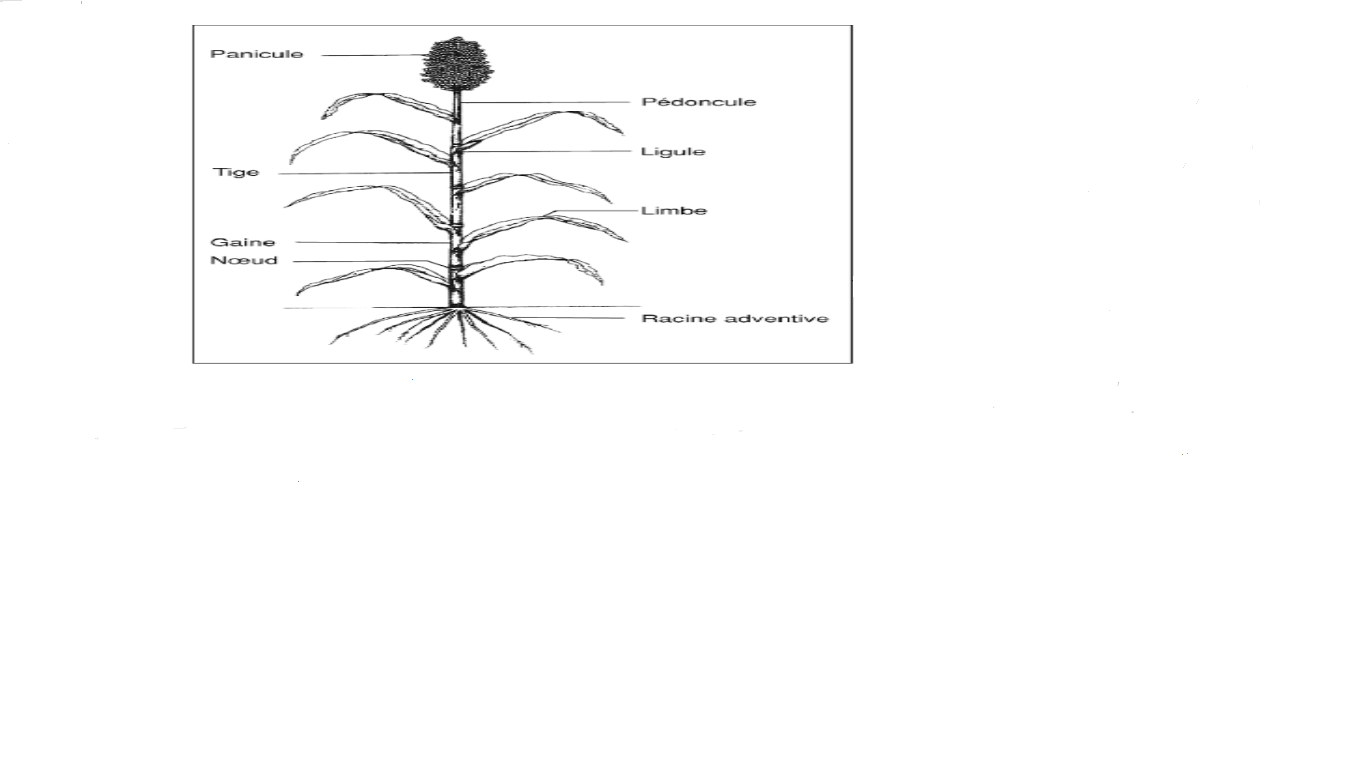
\includegraphics[width=18cm]{images/Schema_Plant_Sorgho}
  \end{center}
\caption{Schéma annoté d’un plant de sorgho (Clerget, 2004)}
\end{figure}


En champ réel les plants de sorgho se présentent ainsi (Fig.~\ref{images/Schema_Plant_Sorgho}):
%(Figure 3):
%% %insérer une image

\begin{figure}%
  \begin{center}
    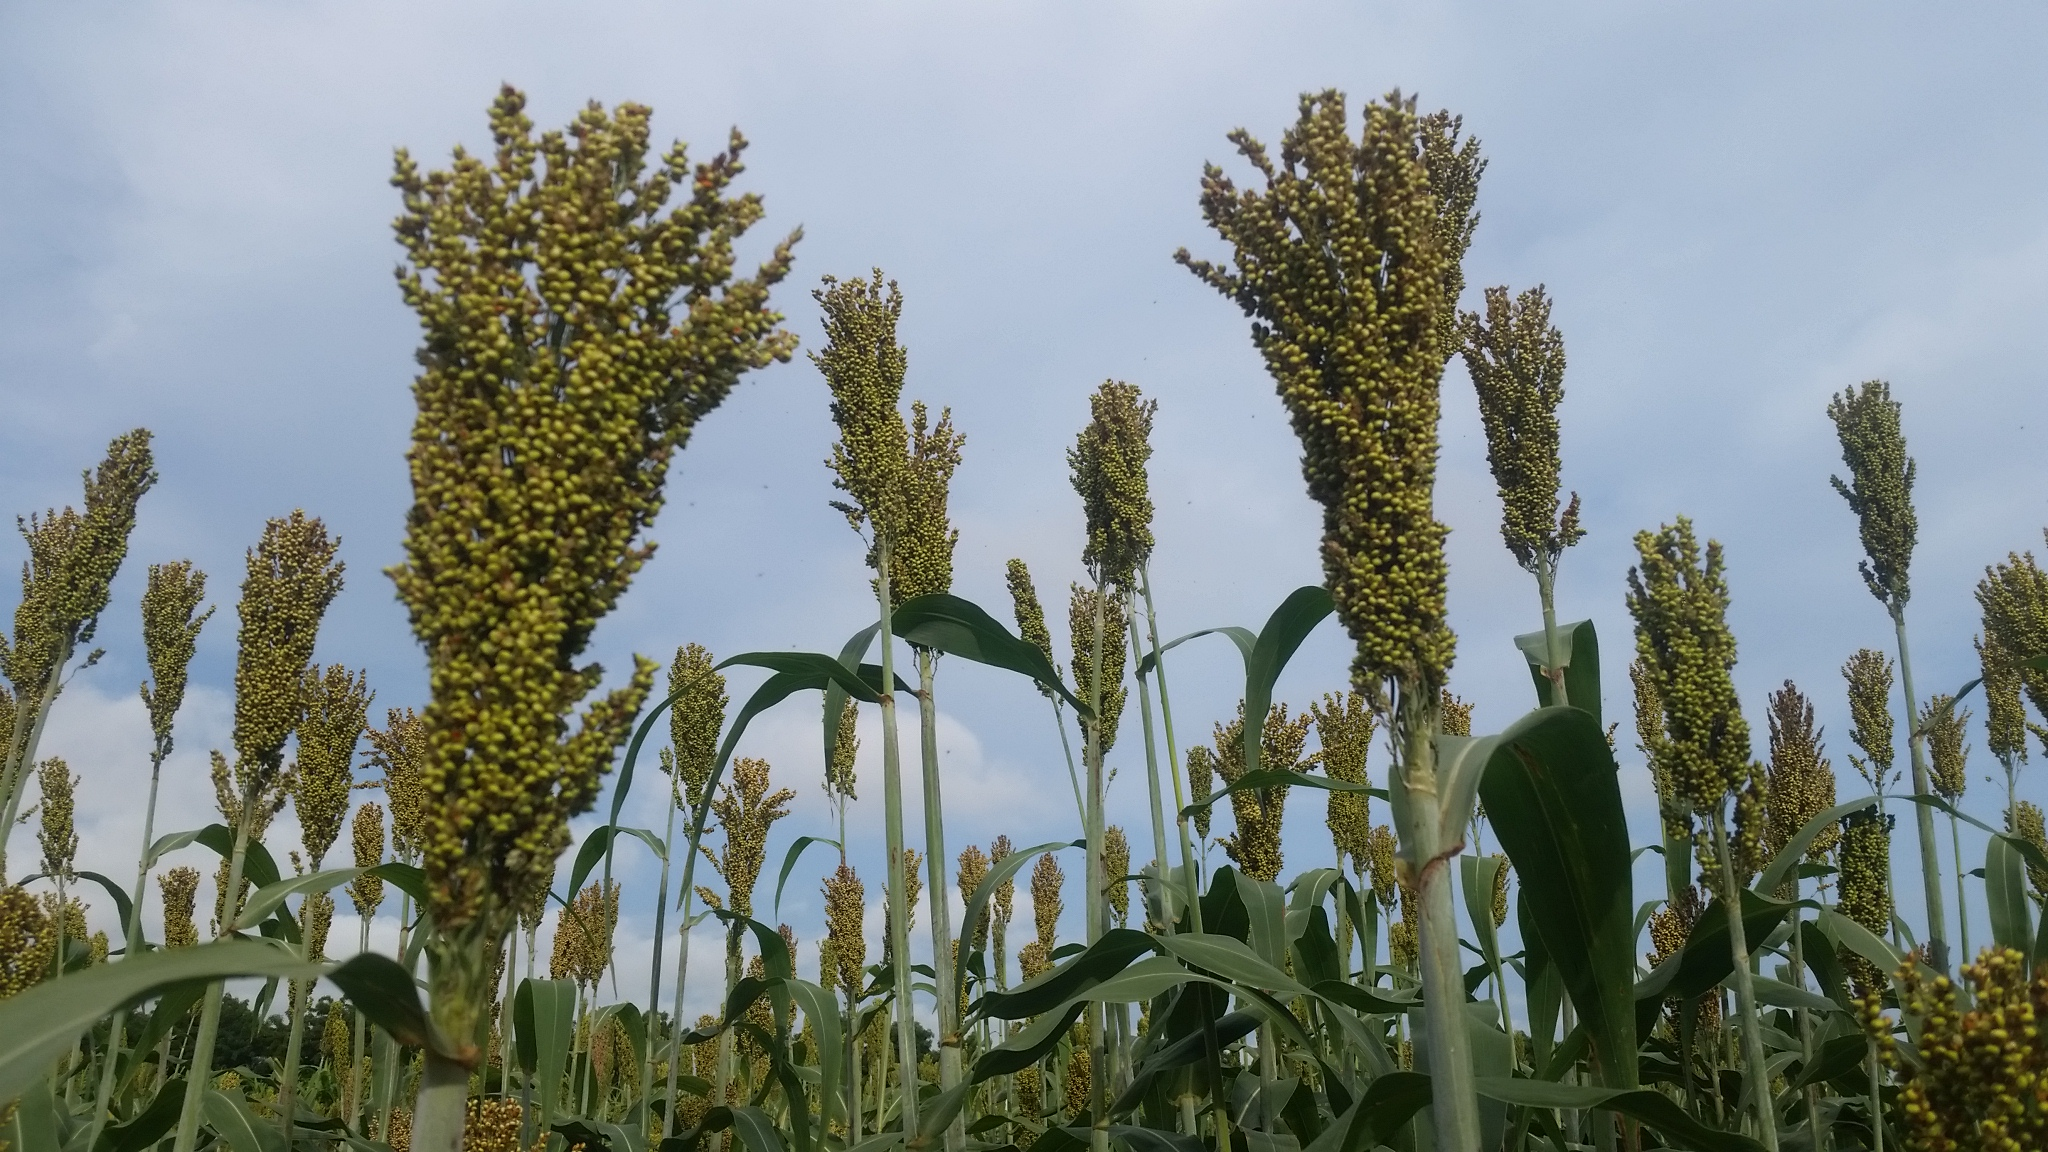
\includegraphics[width=10cm]{images/PlantDeSorgho}
  \end{center}
\caption{Représentation de plants de sorgho en champ réel}
\end{figure}

Par ailleurs, en 2013 Jacques CHANTERAU et al, résument les
différentes races du sorgho et leurs caractéristiques d'identification
(Tableau 1)\footnote{Google books}:

%% https://books.google.sn/books?d=3RFaAgAAQBAJ&pg=PA16&lpg=PA16&dq=sorgho+botanique&source=bl&ots=00CcJJ96PK&sig=QVuYL1AdbFVLs8ewE2B_2Gau_to&hl=fr&sa=X&ved=0ahUKEwjvv7rm2evYAhWBtBQKHekaBpkQ6AEIajAP#v=onepage&q=sorgh\%20botanique&f=false
%%   %insérer un tableau
%%   Tableau 1: Principaux caractères identitaires des races du sorgho.

L’inflorescence est une panicule de forme variable. Le grain est\,un
caryopse de couleur variable (blanche, rouge, brune et jaune), qui, à
maturité, est plus ou moins dégagé des glumes (Saint-Clair, 1989\,;
Chanterau et Nicou, 1991).  Tout comme le maïs et la canne à sucre, le
sorgho appartient à la tribu des Andropogoneae. Les Andropogoneae sont
en effet, une tribu de plantes monocotylédones de la famille des
Poaceae et de la sous-famille des Panicoïdeae.

La classification (cladogramme) phylogénétique des Poaceae dont fait
partie le sorgho, se présente comme suit (Figure 4):

%%   %insérer une image


\begin{figure}%
  \begin{center}
    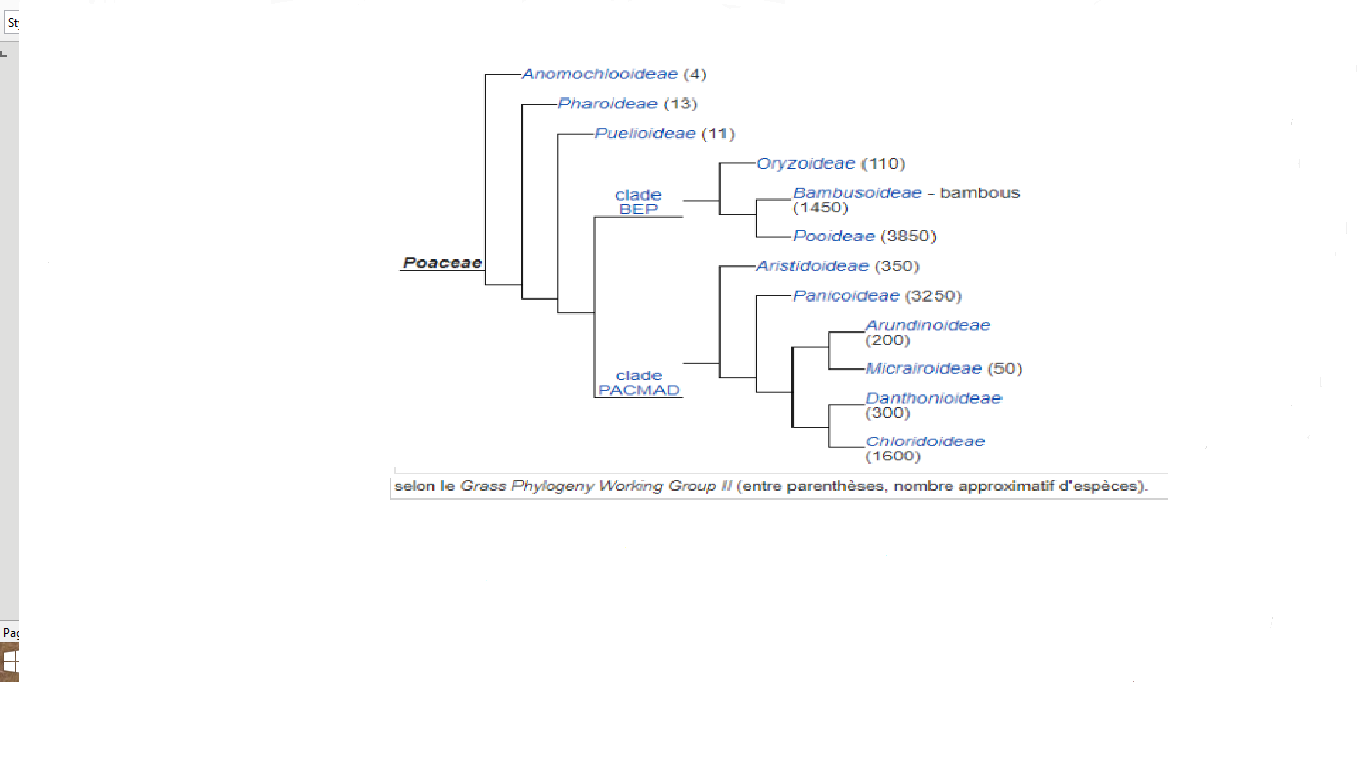
\includegraphics[width=10cm]{images/PhylogenyPoacea}
  \end{center}
\caption{Classification phylogénétique des Poaceae.}
\end{figure}


Le clade BEP (ou BOP) regroupe les Bambusoideae, Oryzoideae et
Pooideae; le second appelé clade PACMAD (ou PACCMAD) regroupe les
Panicoideae, Arundinoideae, Chloridoideae, Micrairoideae,
Centothecoideae, Aristidoideae et
Danthonioideae\footnote{https://fr.wikipedia.org/wiki/Poaceae}.

\subsection{Écologie:}

\subsubsection\,Photosensibilité\,(lumière):
Le sorgho est une plante de jours
courts qui réagit de diverses façons à la photopériode. À des
latitudes élevées, certains cultivars tropicaux ne fleurissent pas ou
ne produisent pas de graines. Aux États-Unis, en Australie et en Inde,
on a noté l’existence de cultivars moyennement sensibles à quasiment
insensibles à la photopériode\cite{BARRO_KONDOMBO_2010}.

\subsubsection\,Conditions écologiques:

 \begin{itemize}
  \item Conditions thermiques:
Le sorgho tolère des températures de tous niveaux. En effet, la sélection a permis de créer
des variétés cultivables en zones tempérées. Là où il ne gèle pas, le
sorgho continue à pousser et à produire de nouvelles feuilles vertes
tant que l’humidité du sol persiste. Il stoppe sa croissance sous les
8\,\degree{}C et meurt lorsque la température passe sous les
3\,\degree{}C\footnote{https://jardinage.ooreka.fr/plante/voir/2001/sorgho}. Il
est largement cultivé dans les régions tempérées et sous les tropiques
jusqu’à 2\,300 m d’altitude. La température optimale est de 25 à
31\,\degree{}C, mais des températures aussi faibles que 21\,\degree{}C
n’ont pas d’incidence grave sur la croissance et le rendement. Mais si
la température nocturne tombe en dessous de 12 à 15\,\degree{}C au
cours de la période de floraison, cela peut entraîner la stérilité. Le
sorgho est sensible au gel, mais moins que le maïs, et de légères
gelées nocturnes pendant la période de maturation provoquent peu de
dégâts.

 \item\,Conditions hydriques:
 Le sorgho est une plante des milieux tropicaux chauds et semi-arides
 qui sont trop secs pour les maïs modernes, mais il existe aussi des
 maïs de zones sèches. Il est particulièrement adapté à la sécheresse
 en raison d’un ensemble de caractéristiques morphologiques et
 physiologiques, notamment un système racinaire étendu, la pruine de
 ses feuilles qui limite ses pertes en eau (figures 1, 2 et 3), et une
 aptitude à interrompre sa croissance pendant les périodes de
 sécheresse et à la reprendre une fois le stress disparu. Le sorgho
 est une plante monocotylédone de la tribu des Andropogoneae. Toutes
 les espèces de cette tribu présentent une photosynthèse en C4, ce qui
 les rend compétitives dans des conditions de chaleur et de fort
 éclairement: ce sont des plantes dites en C3, la plante du sorgho
 dite plante en C4, a un avantage compétitif dans ce sens
 où\,lorsqu’elle est soumise à la sécheresse, à la chaleur et à un
 faible taux d’azote (N2) ou de dioxyde de carbone (CO2) et
 lorsqu’elle est cultivée par exemple dans un environnement à
 30\,\degree{}C, elle perd moins de molécules d’eau (les graminées en
 C3 perdent environ 833 molécules d’eau par molécule de CO2 fixée
 tandis que le sorgho en perd seulement 277). Ceci offre donc un
 avantage aux plantes en C4 (sorgho) dans les environnements
 arides\footnote{\url{https://fr.wikipedia.org/wiki/Fixation_du_carbone_en_C4}}
 (zone sahélienne au Burkina Faso). Des précipitations de 500 à 800 mm
 également réparties pendant la saison de production conviennent
 généralement aux cultivars qui mûrissent en 3 à 4 mois. Le sorgho
 tolère un certain niveau d’asphyxie racinaire et on peut le faire
 pousser dans des zones à fortes précipitations.

 
 \item~Conditions édaphiques:
  Le sorgho est bien adapté sur les vertisols lourds (en pédologie ou science du sol,
 le\,vertisol\,est un sol riche en argile du type 2/1 c’est-à-dire
 contenant une couche d’oxyde d’aluminium enserrée par deux couches de
 tétraèdres de
 silice\footnote{https://fr.wikipedia.org/wiki/Vertisol} que l’on
 trouve couramment dans les tropiques, où sa tolérance à l’asphyxie
 racinaire est souvent nécessaire, mais les sols sableux légers lui 
conviennent tout autant. C’est toutefois sur les limons et les limons
 sableux que sa culture réussit le mieux. La fourchette de pH du sol
 supportée par le sorgho est de 5.0 à 8.5, et il tolère davantage la
 salinité que le maïs (6 à
 7.5)\footnote{\url{http://www.bioactualites.ch/fileadmin/documents/bafr/production-vegetale/grandes-cultures/4.5\.11\-73_Mais.pdf}}. Il est adapté aux sols pauvres et peut produire du grain sur des sols où beaucoup d’autres cultures échoueraient.
 
 \end{itemize}
 
\subsection{Morphologie et biologie:} La plante du sorgho
(Sorghum bicolor ou S.bicolor) comprend une tige principale
accompagnée de talles issues du développement de bourgeons
adventifs sur le collet du maître brin. La hauteur de la plante à
maturité varie beaucoup (de 50cm à plus de 5m). En fonction des
cultivars et de leur situation, les feuilles (alternes, longues,
retombantes, vert clair ou vert foncé) portées par les tiges
varient en nombre (de quelques unités à plus de 30): figures
1,2,3.[2] Le S.bicolor est principalement autogame, mais une
pollinisation croisée par le vent peut se produire dans certaines
conditions, à plus de 60\% selon le génotype, et en moyenne
environ 6\% (Ellstrand et Foster, 1983; House, 1985; Perdersen et
al, 1998; Schertz et Dalton, 1980). Puisque l’espèce se reproduit
à la fois par autopollinisation et par pollinisation croisée, la
plupart des races locales de sorgho cultivées par les
agriculteurs de subsistance sont constituées de mélanges de
lignées pures et de lignées partiellement pures (Singh et al,
1997). Le degré d’allogamie varie notamment en fonction du type
de panicule du cultivar; généralement, la pollinisation croisée
est plus élevée dans le cas des sorghos herbeux à panicule lâche
que dans celui des sorghos cultivés à panicule compacte. Selon
certaines estimations, le taux d’allogamie chez le sorgho cultivé
en plein champ varie de 5 à plus de 40\% (Barnaud et al., 2008;
Djè et al., 2004; Doggett, 1988; Ellstrand et Foster, 1983;
Schmidt et Bothma, 2006). Plusieurs espèces de pollinisateurs ont
été observées consécutivement visitant des fleurs de sorgho
cultivé (Immelman et Eardley, 2000; Schmidt et Bothma,
2006). Lors de la collecte des insectes, des grains de pollen de
sorgho ont été trouvés sur chacun de ceux-ci. Cependant, il n’a
pas été déterminé si le déplacement des insectes occasionnait une
pollinisation croisée. D’autres études doivent être réalisées
pour déterminer l’importance de la pollinisation par les insectes
chez le S. bicolor. La floraison et la pollinisation du S.bicolor
sont décrites dans House (1985), Singh et al. (1997) et Srinivasa
Rao et al (2013). L’inflorescence commence à se former 30 à 40
jours après la germination. Le sorgho cultivé fleurit
généralement 55 à 70 jours après la germination en climats
chauds, mais, selon le génotype, la plante peut fleurir 30 à 100
jours après la germination. Le temps humide et frais peut
retarder la floraison. Les fleurs commencent à s’ouvrir deux
jours après que l’inflorescence a émergé de la gaine. Les
épillets (subdivisions de l’inflorescence qui comportent
plusieurs fleurs) sessiles, situés au sommet de l’inflorescence,
sont les premiers à fleurir, puis la floraison se poursuit vers
le bas de l’inflorescence durant 4 ou 5 jours. Chaque panicule
peut comprendre jusqu’à 6000 fleurons (Quinby et Karper,
1947). La floraison ne survient pas au même moment chez toutes
les inflorescences dans un champ, de sorte que le pollen est
généralement présent durant 10 à 15 jours. Le moment de la
floraison varie en fonction du génotype et du climat, mais
celle-ci se produit généralement du milieu de la nuit au milieu
de la matinée et atteint son maximum vers le lever du soleil. Le
gonflement des lodicules facilite l’ouverture des fleurs. Lorsque
les stigmates deviennent visibles, le filet des étamines
s’allonge, et les anthères deviennent pendantes. Une fois que les
anthères sont sèches, le pore apical s’ouvre et le pollen est
libéré. La majeure partie du pollen d’une inflorescence fertilise
les ovules de la même inflorescence. La pollinisation croisée est
possible lorsque le pollen est transporté dans les airs. Le
stigmate est pollinisé avant que les anthères émergent des
épillets. Les grains de pollen sont transportés jusqu’au stigmate
et germent. Un tube pollinique se forme, et le grain de pollen
divisé en deux noyaux descend dans le style pour aller fertiliser
l’ovule. Un noyau spermatique fertilise l’ovule et produit un
embryon 2n, et l’autre noyau fusionne avec les noyaux polaires
pour produire un albumen 3n. Après la pollinisation, les glumes
se referment, et les anthères et stigmates vides en dépassent
généralement. Certaines variétés à glumes longues sont
cléistogames (les fleurons ne s’ouvrent pas pour la
fertilisation). Les stigmates non fécondés demeurent réceptifs
jusqu’à 16 jours. Après la fertilisation, la différenciation des
organes se déroule sur environ 12 jours. Les graines passent par
trois stades de développement, laiteux, pâteux mou et pâteux dur,
et parviennent à maturité en environ 30 jours. Le S.bicolor se
reproduit par ses graines.
  
\subsection{Intérêt et utilisation du sorgho:}

Sorghum bicolor (L.) Moench est une céréale importante,
particulièrement pour les zones chaudes à pluviométrie réduite de la
zone tropicale. Le sorgho occupe le cinquième rang des plus
importantes céréales dans le monde, qu’il s’agisse du volume de la
production ou des superficies cultivées (FAO et ICRISAT, 1997).En
Afrique subsaharienne, le sorgho est la deuxième céréale en importance
après le maïs. Le Nigeria en est le premier producteur de la région
avec 7\% de la production mondiale (FAO, 1995). Le sorgho est la
principale céréale cultivée au Burkina Faso, avec plus d’un million et
demi d’hectare (Cirad, 2016).C’est la plus importante culture vivrière
dans les régions tropicales semi-arides d’Afrique. Selon Dahlberg et
al, le sorgho est l’aliment de base de 500 millions de personnes dans
plus de 30 pays de la zone tropicale semi-aride\footnote{ma note de
bas de page}. Au Burkina Faso, le sorgho est la céréale la plus
répandue, sa culture y est pratiquée partout en saison des pluies, là
où les précipitations sont supérieures aux valeurs 400 à 500 mm. La superficie
consacrée à la culture du sorgho est passée de 1 016 275 ha en 2000 à
1 619 590 ha en 2007 (FAO, 2009) et couvre actuellement 1,80 millions
d’Hectares (USDA, 2016). Dans les régions tropicales, le sorgho est
essentiellement cultivé pour son grain destiné d’abord à
l’alimentation humaine. Le grain peut être consommé entier ou
décortiqué et réduit en poudre pour faire la bouillie, le tô (nom d’un
des plats locaux cuisiné sous forme de pâte dans plusieurs pays
d’Afrique subsaharienne dont le Burkina Faso), du couscous et des
beignets. Le grain peut être fermenté pour donner des boissons
alcoolisées: bière (dolo) ou du vin de sorgho (Mémento de l’agronome,
1991).Les résidus de récolte, soit l’ensemble des tiges, feuilles et
panicules égrenées, représentent pour l’agriculteur une importante
source de fourrage pour l’alimentation de son bétail (Chantereau et
Nicou, 1991). Les graines (entiers) sont fournies directement aux
volailles. Les tiges sont employées pour la confection des nattes,
dans la construction des maisons (matériaux de construction pour
réaliser des palissades) et des enclos ou comme combustible
(Saint-clair, 1989)[3]D’autres utilisations du sorgho sont à
signaler: la paille (feuilles et tiges) sert comme fourrage. Les
tiges de certains sorghos bicolor sont consommées en frais comme la
canne à sucre. Les cendres servent à la préparation de la potasse
alimentaire. La moelle de sorgho est utilisée comme support pour les
coupes anatomiques. Certains sorghos à forte coloration tannique
servent dans la teinture du cuir. Les extraits de composés phénoliques
servent en cosmétique pour le bronzage. Si dans les principales
régions productrices d’Afrique et d’Asie, plus de 70\% du sorgho sont
consommés par l’Homme, en Amérique du Nord, Amérique centrale,
Amérique du Sud et Océanie par contre la plus grande partie de la
production sert à l’alimentation animale.[2]La culture a également une
vocation industrielle orientée sur la production de la pâte à papier,
la production du fuel, etc\footnote{ma note de bas de page}.En
novembre 2016, l’USDA (Unitites States Department of Agriculture) a
résumé les situations africaine et mondiale de production du sorgho:
%%   (tableau 1):

%%   %insérer un tableau

%%   Tableau 2: Situations africaines et mondiale de production du sorgho, selon l’USDA; p.: désigne la production réelle et est.: représente les estimations.
\section{Productions agricoles de légumineuses: Le niébé i.e Vigna unguiculata (L.) Walp.}
%%   %insérer l'image ( figure 5)
\begin{figure}%
  \begin{center}
   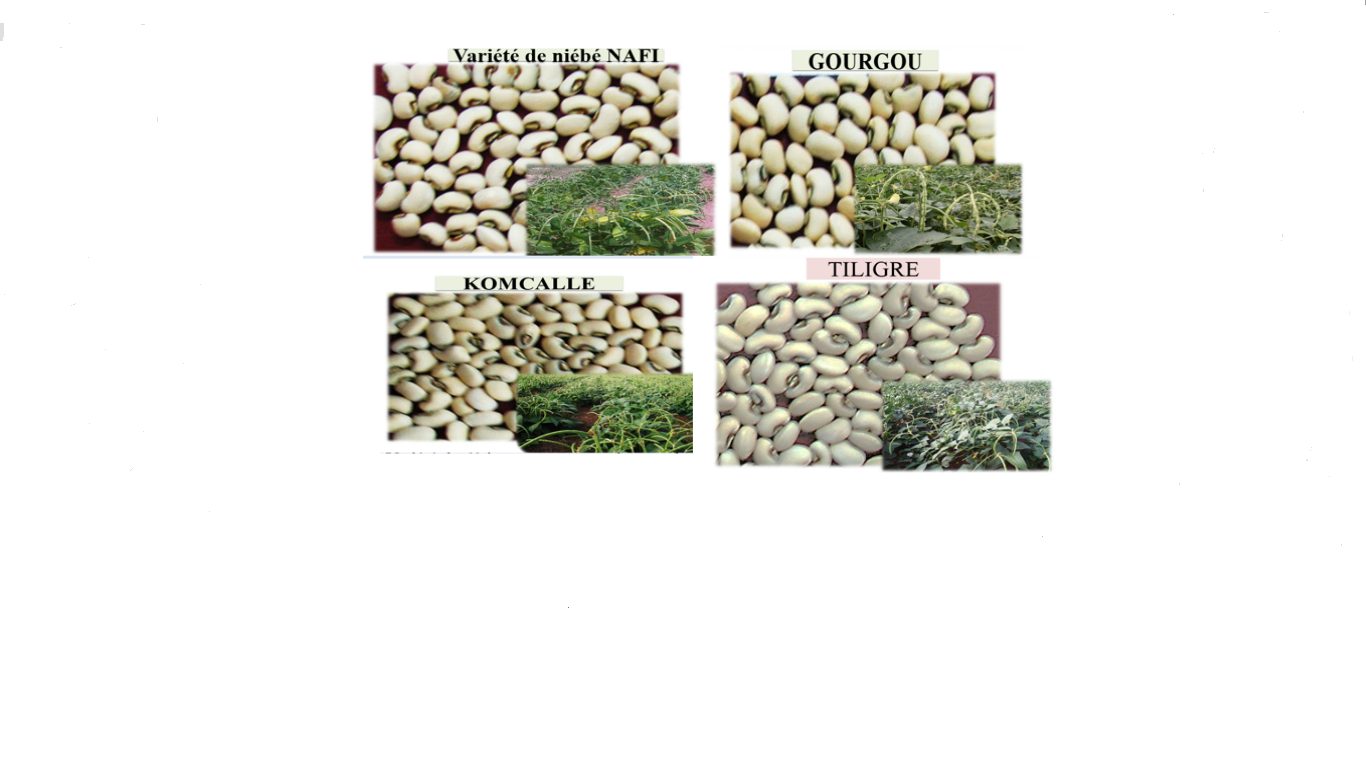
\includegraphics[width=10cm]{images/VariétésdeNiébéauBF}
  \end{center}
\caption{Quelques variétés de niébé au Burkina Faso}
\end{figure}

%%   Figure 5:Quelques variétés de niébé (graines et plantes) observées au Burkina Faso.
%%   \subsection{ Origine et diffusion:}
%%   Le niébé, V. unguiculata est une légumineuse annuelle dont le centre
%%   d’origine était controversé avant les études de Faris (1963;
%%   1965). Piper (1913), a donné une double origine au niébé: l’Inde et
%%   l’Afrique. Faris (1963, 1965), après des études qui se sont reposées
%%   sur une description cytologique et morphologique des formes sauvages
%%   et cultivées du niébé montre que l’Afrique de l’Ouest et plus
%%   probablement le Nigeria est le centre d’origine du niébé. Sa diffusion
%%   vers l’Asie, en parallèle avec celle du sorgho, date de 2300 av
%%   J-C. Le niébé est introduit en Europe vers 300 av J-C où il reste une
%%   culture mineure dans la partie méridionale. Les Espagnols et les
%%   Portugais l’exportent au 17éme siècle vers le nouveau monde. D’autres
%%   cultivars sont transportés directement de l’Afrique vers l’Amérique
%%   latine avec le trafic de l’esclave. Le niébé atteint le Sud des
%%   États-Unis au début du 19éme siècle.[4]

%%   \subsection{Taxonomie:}

%%   Le niébé a été décrit par Linné, à partir d’une forme cultivée
%%   provenant des Antilles, sous le nom de Dolichos unguiculatus, qui
%%   deviendra Vigna unguiculta (Pasquet et Baudouin, 1997). Vigna
%%   unguiculta inclut des formes cultivées et des formes sauvages. Les
%%   formes cultivées se distinguent des formes sauvages par des gousses
%%   indéhiscentes, des graines et des gousses de taille plus importante
%%   (Lush et Evans, 1981). Selon Vanderborght et Baudoin (2001), les
%%   formes cultivées sont regroupées dans la sous-espèce unguiculta,
%%   laquelle est subdivisée en quatre cultigroupes: i) le cultigroupe
%%   Unguiculta (anciennement V.sinensis (L.) Savi ex Hassk), forme
%%   couramment cultivée et plus importante en Afrique; ii) le cultigroupe
%%   Biflora (anciennement V. unguiculta subsp. Cylindrica (L.) Verdcourt),
%%   à petites gousses érigées, cultivé principalement en Asie; Hi) le
%%   cultigroupe Sesquipedalis (anciennement V. unguiculta
%%   var. Sesquipedalis (L.) Ohashi), à gousses très longues et pendantes;
%%   iv) le cultigroupe Texfilis (anciennement V.sinensis var fextilis A
%%   Cheval) avec de long pédoncule est présent en Afrique de l’Ouest. Le
%%   niébé est une dicotylédone de l’ordre des Fabales, famille Fabaceae,
%%   sous famille Faboideae, tribu Phaseoleae, sous tribu Phaseolinae,
%%   genre Vigna et la section Catiang (Verdcourt, (1970); Maréchal et
%%   al. (1978))[4].
%%   Le niébé appartient à:
%%   \begin{itemize} 
%%   \item Règne: Plantae
%%   \item Sous règne: Tracheobionta
%%   \item Division: Magnoliophyta
%%   \item Classe: Magnoliopsida
%%   \item Sous classe: Rosidae
%%   \item Ordre: Fabales
%%   \item Famille: Fabaceae
%%   \item Sous famille: Faboideae
%%   \item Tribu: Phaseoleae
%%   \item Sous tribu: Phaseolineae
%%   \item Genre: Vigna
%%   \end{itemize}
%%   \subsection{ Écologie:}

%%   a. Photosensibilité:

%%   Ce caractère a été largement étudié, en particulier par Steele
%%   (1972). On distingue trois groupes: Le premier groupe,
%%   photo-indépendant tardif, comprend des génotypes indifférents à la
%%   photopériode. La croissance est indéterminée et le port quelquefois
%%   érigé mais le plus souvent volubile. Ces génotypes sont généralement
%%   tardifs et ont une floraison échelonnée à partir de nœuds éloignés au
%%   cours de la saison culturale. On trouve ces cultivars dans les zones
%%   les plus proches de l’équateur comme les savanes guinéennes humides de
%%   l’Afrique, où ils sont cultivés surtout en première saison humide.  Le
%%   deuxième groupe, photo-indépendant précoce, est constitué des
%%   génotypes également indifférents à la photopériode. Ces génotypes
%%   fleurissent précocement à partir des premiers nœuds de la tige
%%   principale et donnent une production groupée, souvent récoltable au
%%   bout de deux mois. Ces variétés sont cultivées dans les zones de
%%   latitude élevée; en Inde, dans le bassin méditerranéen et aux
%%   États-Unis.  Le troisième groupe, photosensible, regroupe des
%%   génotypes sensibles à la photopériode. Le port est généralement
%%   rampant et nettement moins volubile que chez les cultivars du premier
%%   groupe. Ce groupe englobe la plupart des cultivars traditionnels de
%%   l’Afrique soudano-sahélienne cultivés en association avec le sorgho et
%%   le mil.[1] Il est à noter que les deux derniers groupes
%%   photo-indépendant précoce et photosensible sont assez
%%   proches. Cultivés en jours très courts, ils sont indiscernables et les
%%   cultivars photosensibles présentent alors un port érigé et fleurissent
%%   dès les premiers nœuds. En revanche, les deux premiers groupes
%%   photo-indépendant tardif et photo-indépendant précoce sont bien
%%   distincts. Cultivés en jours longs, ils sont tardifs mais leurs ports,
%%   rampant pour l’un et volubile pour l’autre, apparaissent très
%%   différents. De plus, le groupe photo-indépendant précoce et le groupe
%%   photosensible ont relativement peu d’ovules par rapport au groupe
%%   photo-indépendant tardif. Ainsi, ce n’est pas le photopériodisme qui
%%   permet de séparer les cultivars de niébé en deux grands groupes
%%   physiologiques comme le supposait Steele (1972), mais l’aptitude à
%%   fleurir rapidement dès les premiers nœuds de la tige principale dans
%%   des conditions très inductives de jours courts\footnote{ma note de bas
%%     de page}.

%%   b. Conditions écologiques:

%%   i. Conditions édaphiques:

%%   Le niébé se cultive sur les sols sableux à argileux. Il ne supporte
%%   pas l’engorgement et l’acidité du sol. Le niébé croît bien à des pH de
%%   4,5 à 9,0 et réussit à fixer l’azote dans des sols possédants moins de
%%   2\% de matière organique et plus de 80\% de sable (Singh et al,
%%   1997).[1]

%%   ii. Conditions thermiques:

%%   Le niébé est une culture très bien adaptée aux régions arides et
%%   semi-arides. C’est une légumineuse cultivée dans les régions
%%   tropicales et subtropicales.[1] iii. Conditions hydriques:

%%   Le niébé est une plante ayant une certaine adaptation à la
%%   sécheresse. Sa culture est effectuée entre les isohyètes 300mm à
%%   1500mm.[1]

%%   \subsection{Morphologie et biologie:}

%%   –L’appareil végétatif

%%   La tige: la tige du niébé est cylindrique, volubile, quelques fois
%%   glabre et creuse. Elle définit le port de la plante qui peut être
%%   érigé, semi-érigé, buissonnant, ou rampant. Chaque nœud de la tige
%%   porte deux stipules et trois bourgeons axillaires.  Les feuilles: la
%%   première paire de feuille est opposée et monofoliée. Les secondes
%%   feuilles sont alternes et trifoliées comprenant deux folioles opposées
%%   et une foliole terminale.  Les racines: le système racinaire est
%%   pivotant avec de nombreuses ramifications, ce qui confère au niébé une
%%   certaine tolérance à la sécheresse. Les racines portent des nodosités
%%   de bactéries fixatrices d’azote atmosphérique.

%%   –L’appareil reproducteur

%%   L’inflorescence: elle est un racème axillaire. Le pédoncule a une
%%   longueur variable, au bout duquel se trouve le rachis. La coloration
%%   des fleurs varie du blanc au violet en fonction de la concentration
%%   d’anthocyanine. Le niébé est une plante autogame (Fery, 1985). Le
%%   cycle des variétés est déterminé au stade 50\% de floraison (Drabo,
%%   1981).  Les fruits: le fruit du niébé est une gousse pendante ou
%%   dressée avec des formes linéaire, spiralée, ou enroulée. La gousse
%%   peut être entièrement pourpre, pigmentée sur les valves à son
%%   extrémité, marbrée ou dépourvue de pigments.  Les graines: la graine
%%   du niébé comporte un tégument qui peut être ridé ou lisse. Elle est de
%%   couleur, de taille, et de forme variables. La graine est riche en
%%   protéines et en carbohydrates.[1]

%%   \subsection{Intérêt et utilisation du niébé:}
%%   Le niébé est un légume africain. Le terme niébé est un mot wolof
%%   désignant une plante légumineuse, le Vigna unguiculata. Le niébé est
%%   une légumineuse herbacée tropicale. Sa culture présente des retombées
%%   économiques, nutritionnelles, et agronomiques considérables. Sur le
%%   plan économique: le niébé est une source de devises pour les pays
%%   producteurs. Les graines du niébé alimentent les échanges économiques
%%   au niveau régional et sous régional. Selon Langyintuo et al, (2003) le
%%   Niger, le Burkina Faso, le Bénin, le Mali, le Cameroun, le Tchad, et
%%   le Sénégal sont les principaux pays exportateurs du niébé; tandis que
%%   le Nigeria, le Ghana, le Togo, la Côte d’ivoire, le Gabon, et la
%%   Mauritanie sont les pays importateurs. En plus du commerce des graines
%%   du niébé, le fourrage est aussi commercialisé et utiliser dans
%%   l’alimentation des animaux. En Afrique occidentale et centrale, le
%%   commerce du fourrage du niébé permet une augmentation de 25\% du
%%   revenu annuel des paysans (Quin, 1997). Sur le plan nutritionnel: les
%%   jeunes feuilles, les gousses immatures, et les graines sont utilisées
%%   dans l’alimentation humaine. La valeur nutritionnelle des graines est
%%   élevée avec en moyenne 23 à 25\% de protéines et 50 à 67\% d’amidon,
%%   ce qui confère au niébé un rôle important dans la lutte contre la
%%   déficience protéique chez les enfants (Quin, 1997). Le niébé a une
%%   valeur nutritionnelle supérieure aux céréales comme le mil, le maïs et
%%   le sorgho. Source de protéines moins coûteuse que celle d’origine
%%   animale (viande, poisson, œuf), le niébé peut contribuer de manière
%%   significative à la solution du problème de déficit protéique souvent
%%   constaté en Afrique. De plus, les fanes de niébé sont un aliment
%%   apprécié des animaux domestiques (Bambara et al, 2008). La graine du
%%   niébé est riche en lysine mais déficiente en acide aminé soufré. Sur
%%   le plan agronomique: la culture du niébé permet un enrichissement du
%%   sol en azote par l’intermédiaire de bactéries fixatrices d’azote
%%   atmosphérique. Quin (1997), montre qu’un hectare de niébé rapporte
%%   40-80 Kg d’azote dans le sol. De par sa croissance rapide, le niébé
%%   assure une couverture du sol,le protégeant ainsi contre l’érosion et
%%   contre l’envahissement des adventices.[1]
%%   \section{Les sols en Afrique subsaharienne: focus sur le Burkina Faso}

%%   Généralités:

%%   Le sol constitue le réservoir où les plantes puisent l’eau et les
%%   éléments minéraux nécessaires à leurs besoins. La capacité de ce
%%   réservoir dépend non seulement des caractéristiques du sol, mais aussi
%%   de la profondeur exploitable par les racines, d’où la notion de
%%   réserve utile racinaire (RUR). La texture et surtout la structure du
%%   sol jouent un rôle important dans la dynamique de l’enracinement des
%%   cultures (Chopart, 1980). La structure détermine aussi la masse
%%   volumique sèche (densité apparente) du sol et par conséquent la
%%   porosité. Les propriétés physiques du sol déterminent également ses
%%   caractéristiques hydrodynamiques, notamment la perméabilité, la
%%   capacité au champ, le point de flétrissement permanent et la réserve
%%   en eau utile\footnote{reference}

%%   %inserer une image

%%   Figure 6: Carte pédologique du Burkina Faso (Haute Volta)\footnote{ma note de bas de page}

%%   À partir des travaux de l’ORSTOM (Boulet, 1976) synthétisés par Fontès
%%   et Guinko (1995), on peut distinguer 8 principaux types de sols au
%%   Burkina. Ce sont: les sols ferrugineux lessivés, les sols peu évolués
%%   d’érosion, les sols bruns eutrophes, les vertisols, les sols
%%   ferrallitiques, les sols halomorphes, les sols hydromorphes et les
%%   sols minéraux bruts. Les deux premiers types de sols occupent plus des
%%   deux tiers du pays.  Les sols ferrugineux lessivés couvrent les plus
%%   grandes étendues. Ils sont localisés essentiellement dans la partie
%%   méridionale de la pénéplaine précambrienne, au sud du 13e
%%   parallèle. Ce sont des sols à texture variable, généralement à
%%   tendance sableuse dans les horizons de surface et argileuse dans les
%%   horizons plus profonds (>40 cm). Ils ont un régime hydrique
%%   imparfait, en rapport avec de mauvaises propriétés physiques (porosité
%%   et perméabilité). Ils ont tous une faible capacité d’échange
%%   cationique. Ils sont régulièrement associés à des sols
%%   gravillonnaires.\footnote{reference} Les sols peu évolués
%%   d’érosion sont plutôt situés dans la moitié nord du pays. Ils sont
%%   installés sur des granites et des migmatites dont ils dérivent. Ils
%%   présentent un horizon sableux en surface (15 à 20cm) et un horizon
%%   argileux au-delà. La compacité et l’imperméabilité de ce second
%%   horizon jouent un rôle néfaste pour l’alimentation hydrique et
%%   l’enracinement.  Les sols hydromorphes sont installés sur des
%%   alluvions fluviatiles ou sur des matériaux d’altération fins. De
%%   faible drainage, ils s’engorgent régulièrement en saison des
%%   pluies. Ils sont surtout développés dans l’ouest du pays et s’alignent
%%   avec le réseau hydrographique majeur: vallées du Mouhoun, du Nazinon
%%   et du Nakambé.  Les sols bruns eutrophes sont caractérisés par une
%%   fraction argileuse importante. La présence d’argile gonflante leur
%%   confère une forte capacité d’échange et un taux de saturation
%%   élevé. Ce sont des sols généralement bien drainés. Leur structure de
%%   surface est variable, de grumeleuse à prismatique. C’est cette
%%   propriété qui règle leur fertilité. Ils sont répartis sur l’ensemble
%%   du territoire, par tâches de faible étendue.  Les vertisols possèdent
%%   la même parenté texturale que les sols bruns. Ils s’en distinguent par
%%   la structure prismatique de leur horizon B. Ce caractère est lié à
%%   leur position topographique basse. De fait, ce sont des sols beaucoup
%%   moins drainés. Ils sont particulièrement développés dans le sud-est et
%%   le centre-ouest (vallée du Sourou).  Les sols minéraux bruts sont des
%%   sols de faible profondeur installés sur la roche-mère ou sur des
%%   horizons cuirassés. Ce sont des sols pauvres. La végétation qu’ils
%%   portent est tantôt clairsemée ou au contraire dense à cause de leur
%%   faible aptitude agricole qui les met à l’abri de toute intervention
%%   humaine.  Les sols halomorphes ou salés sont installés au nord du
%%   pays. De texture variée, ces sols ont une structure franchement
%%   dégradée. Ce sont des sols pauvres qui supportent des steppes
%%   arbustives extrêmement lâches.  Les sols ferrallitiques sont localisés
%%   dans le sud-ouest du pays où ils occupent une faible surface. Leur
%%   profil s’apparente à celui des sols ferrugineux, mais leurs propriétés
%%   physiques et chimiques les différencient nettement. Ils constituent de
%%   bons supports pour les cultures et pour la végétation naturelle
%%   dominée par les savanes arborées.
%%   \section{Point sur la situation générale de la dégradation des sols au Burkina Faso}
%%   Pays sahélien, le Burkina Faso est soumis depuis plusieurs décennies à
%%   une forte dégradation de ses ressources naturelles, limitant ainsi le
%%   développement des productions agro sylvopastorales (Thiombiano,
%%   2000). Cela est en relation avec le fait que le pays connaît en
%%   général des conditions climatiques précaires, une croissance
%%   démographique relativement élevée et une baisse continue de la
%%   fertilité des sols. Les sols étant soumis à d’énormes contraintes
%%   climatiques (érosions hydrique et éolienne, amplitudes thermiques,
%%   etc.), deviennent très sensibles à la dégradation et ne supportent
%%   pas, de façon soutenue, les systèmes et modes de production agricole
%%   actuellement pratiqués (PANA, 2003). A titre d’illustration, une étude
%%   de l’INERA (2003) montre que la dégradation affecte de nos jours plus
%%   de 24\% des terres arables au Burkina, ce qui est préjudiciable à
%%   l’économie nationale. Une autre plus récente estime également
%%   qu’environ 11\% des terres du pays sont considérées comme très
%%   dégradées et 34\%, comme moyennement dégradées (SP CONEDD, 2006).  Les
%%   sols du Burkina Faso sont naturellement pauvres en matières organiques
%%   notamment en éléments nutritifs essentiels dont l’azote (N) et le
%%   phosphore (P) (Traoré et Toé, 2008) et ont une faible résistance à
%%   l’érosion (Berger, 1991). Aussi, les pays sahéliens en général et le
%%   Burkina en particulier sont sensibles, vulnérables et en proie à une
%%   diminution accélérée des ressources naturelles et à une aggravation de
%%   la pauvreté dans les zones rurales (Roose, 2004). Les aspects les plus
%%   ressentis par les populations restent la réduction significative de la
%%   couverture végétale avec une crise du bois[1].Au Burkina Faso, étant
%%   donné que moins de 10\% de la population a accès à d’autres sources
%%   d’énergie que le bois de feu, près de 250 000 hectares de forêts sont
%%   défrichés annuellement pour satisfaire les besoins en bois de chauffe
%%   et 75 000 hectares supplémentaires sont convertis en nouveaux
%%   champs. Cette tendance est toujours à l’augmentation. Dans le même
%%   temps, seuls 1000 hectares sont reboisés1. A titre illustratif, les
%%   Mossis, sur les plateaux du Burkina Faso, brûlent les pailles du mil,
%%   faute de bois, et appauvrissent leurs sols déjà épuisés. Les
%%   rendements s’en ressentent, et la solution à court terme consistant à
%%   écourter les périodes de jachère ne pouvant ainsi avoir que des
%%   conséquences catastrophiques à long terme2. A coté de la crise de
%%   bois, s’ajoutent la dégradation des sols avec la perte de
%%   potentialités (d’où une chute des rendements agricoles) et une
%%   diminution des ressources en eaux avec l’assèchement et l’ensablement
%%   des cours d’eau (Zombré, 2006).[1]
%%   \section {Avantage des associations et rotations de légumineuses-céréales:}

%%   De manière schématique, nous pouvons représenter l’association et la rotation culturale comme suit:
%%   %insérer une image
%%   Figure 7: Représentation schématique de l’association et de la rotation culturale

%%   \subsection{ Avantages et intérêts généraux:}
%%   Les deux raisons les plus souvent avancées pour l’adoption des
%%   associations d’espèces résident dans le gain de rendement global par
%%   rapport à des cultures pures (mono spécifiques) et dans l’amélioration
%%   significative et quasi systématique de la teneur en protéines de la
%%   céréale, ceci quelle que soit sa proportion dans le mélange récolté
%%   (Jensen, 1996). Les associations légumineuse-céréale permettent aussi
%%   une meilleure valorisation des ressources du milieu comparativement
%%   aux cultures mono spécifiques correspondantes dans les systèmes à bas
%%   niveaux d’intrants azotés (Bedoussac et Justes, 2010). Les
%%   associations sont également un moyen de réduire, dans certaines
%%   situations, la pression des adventices, maladies et ravageurs
%%   (Altieri, 1999), souvent considérés comme des facteurs déterminants de
%%   la production agricole, faisant ainsi des associations une alternative
%%   positive à la lutte chimique (Hauggaard-Nielsen et al, 2001). Les
%%   mélanges d’espèces présentent aussi d’autres avantages comme: i) la
%%   réduction de l’érosion des sols par une meilleure couverture et
%%   enracinement (Zougmoré et al, 1998); ii) l’amélioration de la
%%   résistance à la verse qui est un accident de végétation atteignant
%%   principalement les céréales, provoqué par la pluie, le vent ou une
%%   attaque de parasites et couchant les tiges au sol.(Anil et al, 1998);
%%   iii) la réduction des risques de lixiviation qui traduit la perte de
%%   nutriments (nitrates) végétaux hydrosolubles du sol, qui sont dissous
%%   et entraînés par les eaux d’infiltration à la suite de pluie ou
%%   d’irrigation (Corre-Hellou 2005) ou encore, iv) la meilleure stabilité
%%   interannuelle des rendements (Lithourgidis et al, 2006). En outre, Chu
%%   et al. (2004) ont aussi montré que le système de culture intercalaire
%%   est très prometteur pour le développement de la production alimentaire
%%   durable dans les conditions de ressources naturelles limitées, et en
%%   particulier dans les situations de ressources limitées en eau (Tsubo
%%   et al, 2005). De ce fait, celles-ci pourraient présenter un intérêt
%%   aussi bien en agriculture biologique qu’en agriculture conventionnelle
%%   pour: i) améliorer la qualité des composantes; ii) réduire les
%%   intrants chimiques; iii) et améliorer les performances économiques et
%%   environnementales des systèmes de production.[1]
%%   Dans le cas spécifique d’association du niébé avec le sorgho, la
%%   plante sorgho aide celle du niébé à se développer (Figure 8: image à
%%   droite).
%%   %insérer image
%%   Les rotations de culture quant à elles consistent à cultiver deux
%%   espèces avec un intervalle de temps i.e faire une suite de cultures
%%   échelonnées au fil des années sur une même parcelle (Figures 7 et
%%   8). Elles constituent également un élément important de la gestion de
%%   la fertilité des sols et des bioagresseurs, et donc représentent un
%%   atout pour l’augmentation des rendements.
%%   \subsection{Biodisponibilité de l’azote dans le sol:}
%%   En effet, par leur capacité à fixer l’azote de l’atmosphère grâce au
%%   processus de la fixation symbiotique, les légumineuses améliorent le
%%   bilan de l’azote dans les systèmes de cultures (Ndakidemi, 2005;
%%   Fustec et al, 2011). Lors de la fixation d’azote atmosphérique, les
%%   légumineuses contribuent à la teneur en N du sol soit en tant que
%%   cultures pures en rotation ou, en association (Bado, 2002; Chu et al,
%%   2004; Ndakidemi, 2005; Makoi et al, 2009). En culture associée par
%%   exemple, les légumineuses peuvent augmenter le statut de N i.e de
%%   l’azote du sol grâce à la fixation et l’excrétion (Trenbath, 1976;
%%   Fustec et al, 2011). De ce fait, les plantes compagnes bénéficient de
%%   la fixation biologique par les légumineuses et le transfert ultérieur
%%   de l’azote des légumineuses aux non-légumineuses. Plusieurs travaux
%%   scientifiques ont signalé que le transfert de l’azote fixé par les
%%   légumineuses symbiotiques à la céréale se fait par l’intermédiaire de
%%   la décomposition et de la minéralisation des racines des légumineuses
%%   et/ou des nodules (Burity et al, 1989) et par les exsudats racinaires
%%   libérés des racines des légumineuses (Ndakidemi, 2005; Makoi et al,
%%   2009). Ce processus est appelé la rhizodéposition (Fustec et al, 2011)
%%   et constitue une source potentielle d’accumulation de l’azote dans le
%%   sol.[1] Par ailleurs, les associations ou rotations de cultures sont
%%   des stratégies qui s’inscrivent bien dans le cadre de
%%   l’intensification écologique puisqu’elles visent à améliorer la
%%   productivité par unité de surface cultivée sans recours à des intrants
%%   supplémentaires. Ce sont des systèmes bien adaptés à la petite
%%   agriculture familiale, car ils peuvent permettre de mieux protéger les
%%   sols, d’en améliorer la fertilité à travers notamment la fixation
%%   symbiotique de l’azote par les légumineuses, de faciliter le contrôle
%%   des mauvaises herbes. Les associations de culture sont aussi une
%%   stratégie de minimisation des risques pour des exploitations soumises
%%   à des températures élevées et des précipitations faibles et souvent
%%   fluctuantes. Optimiser le fonctionnement de ces systèmes qui sont déjà
%%   largement utilisés par les paysans est donc un enjeu fort de
%%   recherche/développement.[6]

\bibliographystyle{plain}
\bibliography{revue_bibliographique}
\end{document}
